\begin{center}
\chapter{{\huge \textbf{Chapter 3}}}
\end{center}
\section{Proposed System}

We put forth a ground-breaking deep learning model that is specially designed for the challenging task of identifying brain anomalies. Our model, which leverages the strength of recurrent neural networks (RNNs) and convolutional neural networks (CNNs), is an industry-level response carefully crafted to handle the complexity of brain imaging data. The architecture of this model expertly navigates the subtleties of many neuroimaging modalities, including as MRI, CT scans, and EEG data. Our model's training is assisted by a curated dataset of annotated brain images using transfer learning for effectiveness and data augmentation for robustness. Our suggested approach sets out to reshape the landscape of medical diagnostics, hoping to hasten accurate detection, enhance treatment planning, and improve patient care. It is supported by an interpretable framework for openness and ethical considerations that prioritize patient privacy.

\subsection{Design}
Our model for detecting brain anomalies was created after careful consideration of the difficulties and complexities involved in applying deep learning to identify anomalies in brain pictures. Our method optimizes the model's capacity to detect abnormalities by combining cutting-edge neural network topologies with domain-specific improvements. The architecture is carefully designed to strike a balance between accuracy and processing efficiency. To provide a comprehensive design approach, we address concerns including model interpretability, training data augmentation, and hyper parameter optimization. Due to the model's adaptability, it can be used in a variety of clinical settings and imaging modalities.

\subsection{Explanation of Different Modules of the Proposed System}
Convolutional and recurrent neural networks are strategically integrated to form the basis of the deep learning model we've suggested. Our model is able to extract spatial features from different brain imaging modalities like MRI and CT scans while deftly collecting temporal patterns in sequential data like EEG signals thanks to this architectural synergy. Data augmentation helps to combat shortage and data preparation guarantees uniformity. Pre-trained CNNs speed up model convergence by utilizing transfer learning. Measures to protect data privacy and diagnostic openness uphold ethical principles. Our model's industry-level capability is confirmed by thorough validation across many datasets, constituting a huge step towards reliable, understandable, and moral brain abnormality detection. Explanation as shown in fig:1 and 2: The model is presented in Figs. 1 and 2 and consists of an ensemble of blocks, each with multiple layers carrying out six fundamental activities, which are Conv2D, MaxPooling2D, Activation, Flatten, Dropout, Dense. The architecture of our model is demonstrated in Figs. 1 and 2. The first layer of the architecture is the input layer, and the input shape is (224, 224, 1) and strides 2. The second layer is a convolution layer with 128 filters. The filter size of this layer is 1 × 1 followed by activation function rule and the 2 × 2 max.
\begin{figure}[h!]
    \centering
    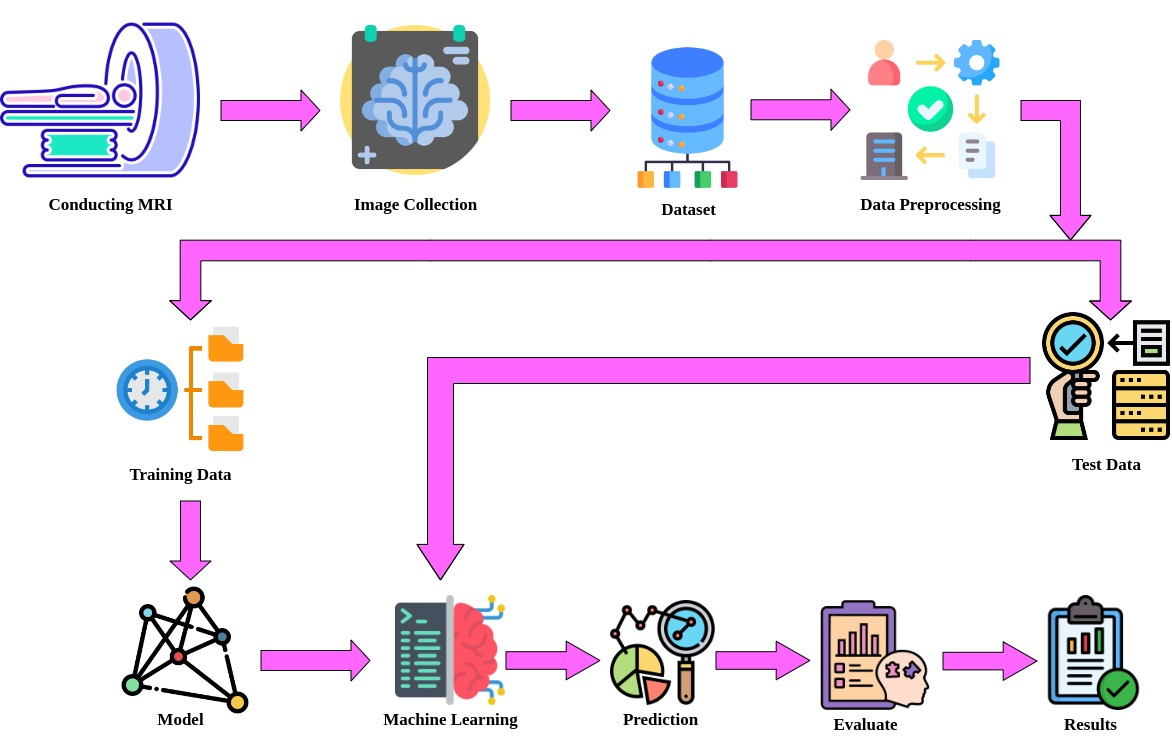
\includegraphics[height=9cm]{img/flowclassification.jpeg}
    \caption{Proposed deep learning flow for classification of brain tumor.}
    \label{fig:classificationImg}
\end{figure}
\begin{figure}[h!]
    \centering
    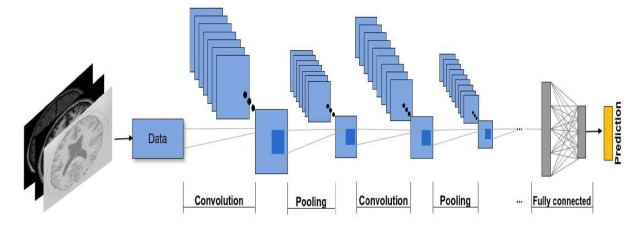
\includegraphics[height=5.5cm]{img/pollingleayer.jpeg}
    \caption{Proposed deep learning architecture for classification of brain tumor pooling layer.}
    \label{fig:pooling}
\end{figure}  \vspace{5mm} \newpage
The next layer of the architecture is a convolution layer with 128 filters. The filter size of this layer is 3 × 3 followed by activation function rule and the 2, 2 maxpooling layer. The next layer of the architecture is a convolution layer with 64 filters. The filter size of this layer is 5 × 5 followed by activation function rule and the 2, 2 maxpooling layer. The next layer of the architecture is a convolution layer with 64 filters. The filter size of this layer is 3 × 3 followed by activation function rule and the 2, 2 max pooling layer. The next layer of the architecture is a convolution layer with 32 filters. The filter size of this layer is 3 × 3 followed by activation function rule Deep Neural Networks for Brain Tumor Detection from MRI Images.

\newpage
\subsection{Summary of the chapter}
The seamless integration of CNNs and RNNs in our cutting-edge deep learning model for brain anomaly detection enables spatial and temporal analysis across several imaging modalities. Data pretreatment and augmentation approaches strengthen this fusion by resolving issues with uniformity and data scarcity. Through pre-trained CNNs, transfer learning speeds up training. Transparent visualizations are produced using an interpretable AI system, while patient data privacy is protected by ethical considerations. Robust validation highlights the strength of our model. In conclusion, the unified architecture of our suggested model, supported by tactical modules, offers the groundwork for precise, open, and moral brain abnormality detection.